\documentclass[tikz,border=4pt]{standalone}
\usepackage{amsmath}
\begin{document}
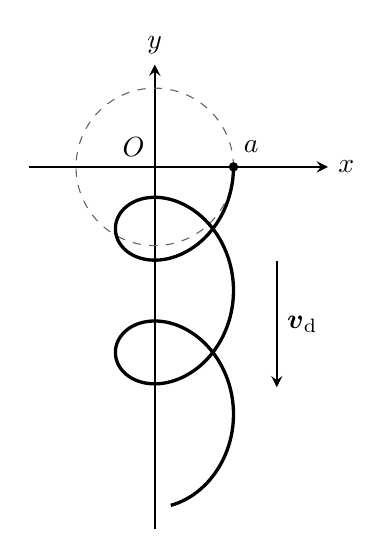
\begin{tikzpicture}[>=stealth, thick, scale=1.0]
  % Axes
  \draw[->] (-1.6, 0) -- (2.2, 0) node[right] {$x$};
  \draw[->] (0, -4.6) -- (0, 1.3) node[above] {$y$};
  \node[above left] at (0, 0) {$O$};

  % Reference circle from (2) (dashed)
  \draw[dashed, thin, black!60] (0, 0) circle (1.0);
  \node[above right] at (1.0, 0.05) {$a$};

  % Trochoid: x(t) = d + (a - d)*cos(t), y(t) = -d*t - (a - d)*sin(t)
  % Choose a = 1.0, d = E/(B*omega) = 0.25 -> a - d = 0.75, t in [0, 4.5*pi]
  \draw[very thick, domain=0:14.2, samples=220]
    plot ({0.25 + 0.75*cos(deg(\x))}, {-0.25*\x - 0.75*sin(deg(\x))});

  % Starting point
  \fill (1.0, 0) circle (0.06);

  % Drift direction arrow
  \draw[->, thick] (1.55, -1.2) -- (1.55, -2.8) node[midway, right] {$\boldsymbol{v}_{\mathrm{d}}$};
\end{tikzpicture}
\end{document}
